\chapter{Limites, continuidad y asintotas}

\begin{theorybox}{Trazabilidad del capitulo}
Este capitulo desarrolla las secciones \texttt{C08.S01-C08.S11} de la matriz de cobertura a
partir de \texttt{sources/Relacion tema 8 (1).pdf}. El hilo conductor es pasar de la lectura
del comportamiento de una funcion a su control algebraico mediante dominios, limites,
continuidad y asintotas.
\end{theorybox}

\section{[C08.S01] Dominio de funciones}

\subsection*{Objetivos de aprendizaje}
\begin{itemize}
  \item Imponer restricciones de existencia en funciones racionales, radicales y logaritmicas.
  \item Escribir el dominio con intervalos y puntos excluidos.
\end{itemize}

\subsection*{Prerrequisitos}
\begin{itemize}
  \item Inecuaciones basicas e interpretacion de intervalos.
\end{itemize}

\begin{theorybox}{Idea minima}
El dominio es el conjunto de valores de \(x\) para los que la expresion tiene sentido. En este
bloque conviene recordar tres reglas basicas:
\[
\frac{1}{g(x)} \text{ exige } g(x)\neq 0,
\qquad
\sqrt{h(x)} \text{ exige } h(x)\geq 0,
\qquad
\ln(k(x)) \text{ exige } k(x)>0.
\]
\end{theorybox}

\begin{methodbox}{Como reconocer y resolver}
\begin{enumerate}
  \item Localiza denominadores, radicales de indice par y logaritmos.
  \item Escribe una condicion de existencia por cada restriccion.
  \item Resuelve el sistema de condiciones y expresa el dominio con intervalos.
\end{enumerate}
\end{methodbox}

\begin{solvedexample}{[EX-C08.S01-01] Dominio con radical y denominador}
Halla el dominio de
\[
f(x)=\frac{\sqrt{x+1}}{x-2}.
\]

\textbf{Desarrollo.} La raiz cuadrada exige
\[
x+1\geq 0 \Longrightarrow x\geq -1.
\]
Ademas, el denominador no puede anularse:
\[
x-2\neq 0 \Longrightarrow x\neq 2.
\]
Por tanto, hay que quedarse con los valores \(x\geq -1\) excluyendo \(x=2\).

\textbf{Respuesta final.}
\[
D_f=[-1,\infty)\setminus\{2\}=[-1,2)\cup(2,\infty).
\]
\end{solvedexample}

\begin{commonerror}{Olvidar que una condicion no sustituye a la otra}
Que una raiz exija \(x\geq -1\) no elimina la necesidad de revisar el denominador. En funciones
mixtas siempre hay que superponer todas las restricciones.
\end{commonerror}

\begin{guidedexercise}{[GX-C08.S01-01] Logaritmo}
Halla el dominio de \(g(x)=\ln(3-x)\).

\textbf{Pista 1.} El argumento del logaritmo debe ser positivo.
\end{guidedexercise}

\begin{shortanswer}{[GX-C08.S01-01]}
\[
D_g=(-\infty,3).
\]
\end{shortanswer}

\begin{fullsolution}{[GX-C08.S01-01]}
\[
3-x>0 \Longrightarrow x<3.
\]
Luego
\[
D_g=(-\infty,3).
\]
\end{fullsolution}

\begin{guidedexercise}{[GX-C08.S01-02] Funcion racional}
Halla el dominio de \(h(x)=\dfrac{1}{x^2-9}\).

\textbf{Pista 1.} Empieza anulando el denominador.
\end{guidedexercise}

\begin{shortanswer}{[GX-C08.S01-02]}
\[
D_h=\R\setminus\{-3,3\}.
\]
\end{shortanswer}

\begin{fullsolution}{[GX-C08.S01-02]}
\[
x^2-9\neq 0 \Longrightarrow (x-3)(x+3)\neq 0.
\]
Por tanto, se excluyen \(x=-3\) y \(x=3\):
\[
D_h=\R\setminus\{-3,3\}.
\]
\end{fullsolution}

\subsection*{Practica autonoma graduada}
\begin{exercise}{[PX-C08.S01-01] Halla el dominio de \(f(x)=x^3-2x+1\).}
\end{exercise}
\begin{exercise}{[PX-C08.S01-02] Halla el dominio de \(f(x)=\dfrac{1}{x-5}\).}
\end{exercise}
\begin{exercise}{[PX-C08.S01-03] Halla el dominio de \(f(x)=\sqrt{x-4}\).}
\end{exercise}
\begin{exercise}{[PX-C08.S01-04] Halla el dominio de \(f(x)=\sqrt{\dfrac{x-1}{x+2}}\).}
\end{exercise}
\begin{exercise}{[PX-C08.S01-05] Halla el dominio de \(f(x)=\ln(x^2-4)\).}
\end{exercise}
\begin{exercise}{[PX-C08.S01-06] Halla el dominio de \(f(x)=\dfrac{\sqrt{9-x^2}}{x+1}\).}
\end{exercise}

\begin{shortanswer}{C08.S01 practica autonoma}
\begin{enumerate}[label=\textbf{PX-C08.S01-\arabic*:}, leftmargin=*]
  \item \(\R\)
  \item \(\R\setminus\{5\}\)
  \item \([4,\infty)\)
  \item \((-\infty,-2)\cup[1,\infty)\)
  \item \((-\infty,-2)\cup(2,\infty)\)
  \item \([-3,-1)\cup(-1,3]\)
\end{enumerate}
\end{shortanswer}

\begin{fullsolution}{C08.S01 practica autonoma}
\begin{enumerate}[label=\textbf{PX-C08.S01-\arabic*:}, leftmargin=*]
  \item Los polinomios estan definidos en todo \(\R\).
  \item Solo se excluye el cero del denominador: \(x\neq 5\).
  \item La raiz exige \(x-4\geq 0\), luego \(x\geq 4\).
  \item Debe cumplirse
  \[
  \frac{x-1}{x+2}\geq 0,\qquad x\neq -2.
  \]
  El estudio de signo da \((-\infty,-2)\cup[1,\infty)\).
  \item El argumento del logaritmo debe ser positivo:
  \[
  x^2-4>0 \Longrightarrow |x|>2.
  \]
  \item La raiz exige \(9-x^2\geq 0\), es decir, \(-3\leq x\leq 3\), y ademas \(x\neq -1\).
\end{enumerate}
\end{fullsolution}

\section{[C08.S02] Lectura de graficas}

\subsection*{Objetivos de aprendizaje}
\begin{itemize}
  \item Extraer de una grafica dominio, imagen, cortes, monotonia y extremos.
  \item Distinguir entre valor de la funcion, tendencia y comportamiento global.
\end{itemize}

\subsection*{Prerrequisitos}
\begin{itemize}
  \item Ejes cartesianos e interpretacion de pares \((x,y)\).
\end{itemize}

\begin{theorybox}{Idea minima}
Leer una grafica no consiste en adivinar una formula, sino en localizar rasgos visibles:
intervalos de definicion, puntos de corte, zonas crecientes o decrecientes, maximos, minimos y
comportamientos destacados.
\end{theorybox}

\begin{methodbox}{Como reconocer y resolver}
\begin{enumerate}
  \item Recorre la grafica de izquierda a derecha.
  \item Anota en que valores de \(x\) esta definida.
  \item Localiza cortes con los ejes y puntos destacados.
  \item Describe donde sube, baja o se mantiene.
\end{enumerate}
\end{methodbox}

\begin{solvedexample}{[EX-C08.S02-01] Leer una parabola en un intervalo}
La siguiente grafica representa una funcion \(f\) en el intervalo \([-1,3]\).

\begin{center}
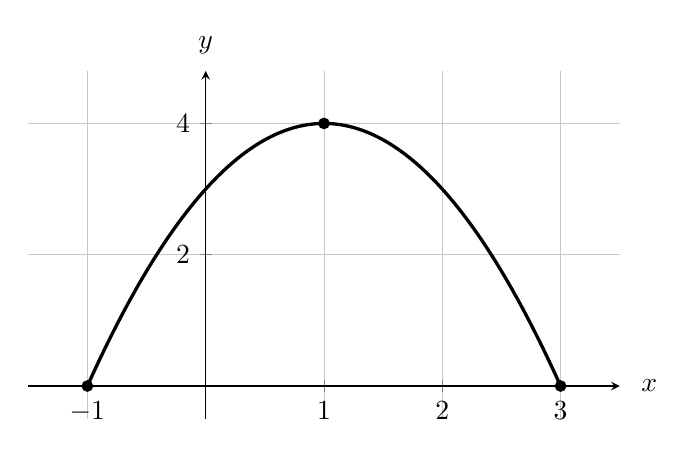
\begin{tikzpicture}
\begin{axis}[
  width=0.75\textwidth,
  height=6cm,
  axis lines=middle,
  xmin=-1.5,
  xmax=3.5,
  ymin=-0.5,
  ymax=4.8,
  samples=120,
  xlabel={$x$},
  ylabel={$y$},
  grid=both,
  grid style={line width=0.1pt, draw=gray!25},
  major grid style={line width=0.2pt, draw=gray!45},
  every axis x label/.style={at={(ticklabel* cs:1.02)},anchor=west},
  every axis y label/.style={at={(ticklabel* cs:1.02)},anchor=south},
]
\addplot[very thick, black, domain=-1:3] {-(x-1)^2 + 4};
\addplot[only marks, mark=*, mark size=1.9pt] coordinates {(-1,0) (1,4) (3,0)};
\end{axis}
\end{tikzpicture}
\end{center}

Indica dominio, imagen, ceros, punto de corte con el eje \(Y\) y donde la funcion es creciente
o decreciente.

\textbf{Desarrollo.} La grafica aparece dibujada desde \(x=-1\) hasta \(x=3\), asi que
\[
D_f=[-1,3].
\]
El punto mas alto es \((1,4)\) y los extremos visibles tocan el eje \(X\) en \((-1,0)\) y
\((3,0)\), luego
\[
\mathrm{Im}(f)=[0,4].
\]
Los ceros son \(x=-1\) y \(x=3\). Para \(x=0\), la grafica corta al eje \(Y\) en \(y=3\),
luego \(f(0)=3\). La funcion sube hasta \(x=1\) y despues baja, de modo que es creciente en
\([-1,1]\) y decreciente en \([1,3]\).

\textbf{Respuesta final.}
\[
D_f=[-1,3],\qquad \mathrm{Im}(f)=[0,4],
\]
\[
\text{ceros: }x=-1,\ x=3,\qquad f(0)=3,
\]
\[
\text{creciente en }[-1,1],\qquad \text{decreciente en }[1,3].
\]
\end{solvedexample}

\begin{commonerror}{Confundir el valor mas alto con el ultimo punto}
El extremo absoluto no tiene por que estar en el extremo derecho de la grafica. Hay que buscar
el punto con mayor o menor altura, no el ultimo que aparece dibujado.
\end{commonerror}

\begin{guidedexercise}{[GX-C08.S02-01] Raices y maximo}
En una grafica se observa que la funcion corta al eje \(X\) en \(-2\) y \(1\), y alcanza un
maximo absoluto en \((0,5)\). Indica sus raices y su valor maximo.
\end{guidedexercise}

\begin{shortanswer}{[GX-C08.S02-01]}
Raices: \(-2\) y \(1\). Valor maximo: \(5\).
\end{shortanswer}

\begin{fullsolution}{[GX-C08.S02-01]}
Las raices son las abscisas de los cortes con el eje \(X\), es decir, \(-2\) y \(1\). El valor
maximo es la ordenada del punto mas alto: \(5\).
\end{fullsolution}

\begin{guidedexercise}{[GX-C08.S02-02] Valor y tendencia}
Una grafica presenta un agujero en \((2,3)\) y un punto relleno en \((2,1)\). Indica \(f(2)\)
y el valor al que tiende la funcion cuando \(x\) se acerca a \(2\).
\end{guidedexercise}

\begin{shortanswer}{[GX-C08.S02-02]}
\[
f(2)=1,\qquad \lim_{x\to 2}f(x)=3.
\]
\end{shortanswer}

\begin{fullsolution}{[GX-C08.S02-02]}
El punto relleno da el valor de la funcion, asi que \(f(2)=1\). El agujero marca el valor al
que se aproxima la grafica por ambos lados, luego
\[
\lim_{x\to 2}f(x)=3.
\]
\end{fullsolution}

\subsection*{Practica autonoma graduada}
\begin{exercise}{[PX-C08.S02-01] Una grafica corta al eje \(Y\) en \(3\) y al eje \(X\) en \(-2\) y \(1\). Indica \(f(0)\) y las raices.}
\end{exercise}
\begin{exercise}{[PX-C08.S02-02] En una grafica el punto mas alto es \((1,4)\) y el mas bajo es \((-2,-1)\). Indica maximo y minimo absolutos.}
\end{exercise}
\begin{exercise}{[PX-C08.S02-03] Una grafica es creciente en \((-3,0)\) y decreciente en \((0,2)\). En que abscisa aparece un maximo local?}
\end{exercise}
\begin{exercise}{[PX-C08.S02-04] En \(x=1\), la grafica se acerca a \(2\) por la izquierda y a \(5\) por la derecha. Existe \(\lim_{x\to 1}f(x)\)?}
\end{exercise}
\begin{exercise}{[PX-C08.S02-05] Una grafica tiene un agujero en \((3,-1)\) y un punto relleno en \((3,2)\). Indica \(f(3)\) y \(\lim_{x\to 3}f(x)\).}
\end{exercise}
\begin{exercise}{[PX-C08.S02-06] Al avanzar hacia la derecha, una grafica se aproxima a la recta \(y=4\). Que comportamiento global se observa?}
\end{exercise}

\begin{shortanswer}{C08.S02 practica autonoma}
\begin{enumerate}[label=\textbf{PX-C08.S02-\arabic*:}, leftmargin=*]
  \item \(f(0)=3\). Raices: \(-2\) y \(1\)
  \item Maximo absoluto \(4\). Minimo absoluto \(-1\)
  \item En \(x=0\)
  \item No existe
  \item \(f(3)=2\) y \(\lim_{x\to 3}f(x)=-1\)
  \item La funcion tiende a una asintota horizontal \(y=4\)
\end{enumerate}
\end{shortanswer}

\begin{fullsolution}{C08.S02 practica autonoma}
\begin{enumerate}[label=\textbf{PX-C08.S02-\arabic*:}, leftmargin=*]
  \item El corte con el eje \(Y\) da \(f(0)=3\); las raices salen de los cortes con el eje \(X\).
  \item Los valores extremos absolutos son las ordenadas del punto mas alto y del mas bajo.
  \item Si primero crece y despues decrece, el cambio se produce en un maximo local en \(x=0\).
  \item Como los limites laterales son distintos, el limite global no existe.
  \item El punto relleno fija el valor de la funcion y el agujero indica la tendencia.
  \item Aproximarse a la recta \(y=4\) para \(x\) grande significa tener una asintota
  horizontal de ecuacion \(y=4\).
\end{enumerate}
\end{fullsolution}

\section{[C08.S03] Limites basicos y laterales}

\subsection*{Objetivos de aprendizaje}
\begin{itemize}
  \item Calcular limites por sustitucion directa cuando no hay indeterminacion.
  \item Estudiar limites laterales cuando el comportamiento cambia a cada lado.
\end{itemize}

\subsection*{Prerrequisitos}
\begin{itemize}
  \item Operaciones algebraicas elementales y valor absoluto.
\end{itemize}

\begin{theorybox}{Idea minima}
Si una expresion es continua en el punto al que tiende \(x\), el limite se obtiene
sustituyendo. Cuando una expresion cambia de signo o de forma segun el lado por el que se
llega, conviene estudiar los limites laterales.
\end{theorybox}

\begin{methodbox}{Como reconocer y resolver}
\begin{enumerate}
  \item Sustituye el valor de \(x\) y comprueba si aparece una expresion bien definida.
  \item Si el comportamiento puede cambiar por la izquierda y por la derecha, separa ambos
  calculos.
  \item El limite global solo existe si los dos laterales coinciden.
\end{enumerate}
\end{methodbox}

\begin{solvedexample}{[EX-C08.S03-01] Laterales que no coinciden}
Estudia
\[
\lim_{x\to 2}\frac{|x-2|}{x-2}.
\]

\textbf{Desarrollo.} Si \(x<2\), entonces \(|x-2|=-(x-2)\), y por tanto
\[
\frac{|x-2|}{x-2}=-1.
\]
Luego
\[
\lim_{x\to 2^-}\frac{|x-2|}{x-2}=-1.
\]
Si \(x>2\), se tiene \(|x-2|=x-2\), asi que
\[
\frac{|x-2|}{x-2}=1.
\]
Entonces
\[
\lim_{x\to 2^+}\frac{|x-2|}{x-2}=1.
\]
Como los laterales no coinciden, el limite global no existe.

\textbf{Respuesta final.}
\[
\lim_{x\to 2^-}\frac{|x-2|}{x-2}=-1,\qquad
\lim_{x\to 2^+}\frac{|x-2|}{x-2}=1,
\]
y por tanto
\[
\lim_{x\to 2}\frac{|x-2|}{x-2}\text{ no existe}.
\]
\end{solvedexample}

\begin{commonerror}{Creer que siempre basta con sustituir}
En expresiones con valor absoluto, funciones a trozos o denominadores que cambian de signo
puede haber comportamientos distintos a izquierda y derecha. Si no se revisan, el limite puede
quedar mal decidido.
\end{commonerror}

\begin{guidedexercise}{[GX-C08.S03-01] Sustitucion directa}
Calcula
\[
\lim_{x\to 1}(3x-2).
\]
\end{guidedexercise}

\begin{shortanswer}{[GX-C08.S03-01]}
\[
1.
\]
\end{shortanswer}

\begin{fullsolution}{[GX-C08.S03-01]}
La funcion es polinomica, asi que basta sustituir:
\[
3\cdot 1-2=1.
\]
\end{fullsolution}

\begin{guidedexercise}{[GX-C08.S03-02] Laterales de una funcion inversa}
Calcula los limites laterales de \(\dfrac{1}{x}\) cuando \(x\to 0\).
\end{guidedexercise}

\begin{shortanswer}{[GX-C08.S03-02]}
\[
\lim_{x\to 0^-}\frac{1}{x}=-\infty,\qquad
\lim_{x\to 0^+}\frac{1}{x}=+\infty.
\]
\end{shortanswer}

\begin{fullsolution}{[GX-C08.S03-02]}
Si \(x\) se acerca a \(0\) por valores negativos, \(1/x\) toma valores negativos de modulo cada
vez mayor. Si se acerca por valores positivos, toma valores positivos cada vez mayores:
\[
\lim_{x\to 0^-}\frac{1}{x}=-\infty,\qquad
\lim_{x\to 0^+}\frac{1}{x}=+\infty.
\]
\end{fullsolution}

\subsection*{Practica autonoma graduada}
\begin{exercise}{[PX-C08.S03-01] Calcula \(\lim_{x\to 2}(x^2+3)\).}
\end{exercise}
\begin{exercise}{[PX-C08.S03-02] Calcula \(\lim_{x\to -1}\dfrac{x^2+1}{x+2}\).}
\end{exercise}
\begin{exercise}{[PX-C08.S03-03] Estudia \(\lim_{x\to 0}\dfrac{|x|}{x}\).}
\end{exercise}
\begin{exercise}{[PX-C08.S03-04] Calcula \(\lim_{x\to 4}\sqrt{x+5}\).}
\end{exercise}
\begin{exercise}{[PX-C08.S03-05] Estudia los limites laterales de \(\dfrac{1}{x-3}\) cuando \(x\to 3\).}
\end{exercise}
\begin{exercise}{[PX-C08.S03-06] Existe \(\lim_{x\to 1}\dfrac{x-1}{|x-1|}\)?}
\end{exercise}

\begin{shortanswer}{C08.S03 practica autonoma}
\begin{enumerate}[label=\textbf{PX-C08.S03-\arabic*:}, leftmargin=*]
  \item \(7\)
  \item \(2\)
  \item No existe
  \item \(3\)
  \item \(-\infty\) por la izquierda y \(+\infty\) por la derecha
  \item No
\end{enumerate}
\end{shortanswer}

\begin{fullsolution}{C08.S03 practica autonoma}
\begin{enumerate}[label=\textbf{PX-C08.S03-\arabic*:}, leftmargin=*]
  \item Sustitucion directa: \(2^2+3=7\).
  \item El denominador no se anula en \(-1\), asi que
  \[
  \frac{(-1)^2+1}{-1+2}=2.
  \]
  \item Por la izquierda vale \(-1\) y por la derecha vale \(1\), luego el limite global no
  existe.
  \item \(\sqrt{4+5}=3\).
  \item Si \(x\to 3^-\), el denominador es negativo y muy pequeno: sale \(-\infty\). Si
  \(x\to 3^+\), sale \(+\infty\).
  \item Es la misma estructura que el ejemplo, con laterales \(-1\) y \(1\), asi que no existe.
\end{enumerate}
\end{fullsolution}

\section{[C08.S04] Limites en el infinito}

\subsection*{Objetivos de aprendizaje}
\begin{itemize}
  \item Comparar crecimientos de polinomios y cocientes racionales.
  \item Reconocer cuando un limite en el infinito tiende a un numero, a \(0\) o a \(\pm\infty\).
\end{itemize}

\subsection*{Prerrequisitos}
\begin{itemize}
  \item Factor comun y comparacion de grados.
\end{itemize}

\begin{theorybox}{Idea minima}
En un cociente de polinomios:
\begin{itemize}
  \item si los grados coinciden, manda el cociente de coeficientes principales;
  \item si el grado del numerador es menor, el limite vale \(0\);
  \item si el grado del numerador es mayor, el limite crece en modulo sin acotacion.
\end{itemize}
\end{theorybox}

\begin{methodbox}{Como reconocer y resolver}
\begin{enumerate}
  \item Identifica los terminos de mayor grado.
  \item Divide numerador y denominador por la potencia mas alta conveniente.
  \item Simplifica y deja que los terminos de grado menor se hagan despreciables.
\end{enumerate}
\end{methodbox}

\begin{solvedexample}{[EX-C08.S04-01] Comparar grados}
Calcula
\[
\lim_{x\to\infty}\frac{2x^2-3}{x^2+x}
\qquad\text{y}\qquad
\lim_{x\to-\infty}\frac{3x-1}{x^2+1}.
\]

\textbf{Desarrollo.} En el primer cociente los grados coinciden, asi que dividimos por \(x^2\):
\[
\frac{2x^2-3}{x^2+x}=\frac{2-\frac{3}{x^2}}{1+\frac{1}{x}}.
\]
Al hacer \(x\to\infty\), los terminos con \(1/x\) desaparecen:
\[
\lim_{x\to\infty}\frac{2x^2-3}{x^2+x}=2.
\]

En el segundo, el grado del numerador es menor que el del denominador. Dividiendo por \(x^2\):
\[
\frac{3x-1}{x^2+1}=\frac{\frac{3}{x}-\frac{1}{x^2}}{1+\frac{1}{x^2}}.
\]
Por tanto,
\[
\lim_{x\to-\infty}\frac{3x-1}{x^2+1}=0.
\]

\textbf{Respuesta final.}
\[
\lim_{x\to\infty}\frac{2x^2-3}{x^2+x}=2,\qquad
\lim_{x\to-\infty}\frac{3x-1}{x^2+1}=0.
\]
\end{solvedexample}

\begin{commonerror}{Quedarse con el termino dominante sin cuidar el signo}
Cuando el infinito es negativo, las potencias impares y pares se comportan de forma distinta.
No basta con mirar el grado: tambien hay que controlar el signo del termino principal.
\end{commonerror}

\begin{guidedexercise}{[GX-C08.S04-01] Grados iguales}
Calcula
\[
\lim_{x\to\infty}\frac{5x-2}{x+3}.
\]
\end{guidedexercise}

\begin{shortanswer}{[GX-C08.S04-01]}
\[
5.
\]
\end{shortanswer}

\begin{fullsolution}{[GX-C08.S04-01]}
Los grados coinciden, asi que manda el cociente de coeficientes principales:
\[
\lim_{x\to\infty}\frac{5x-2}{x+3}=5.
\]
\end{fullsolution}

\begin{guidedexercise}{[GX-C08.S04-02] Numerador de menor grado}
Calcula
\[
\lim_{x\to\infty}\frac{4}{x^2+1}.
\]
\end{guidedexercise}

\begin{shortanswer}{[GX-C08.S04-02]}
\[
0.
\]
\end{shortanswer}

\begin{fullsolution}{[GX-C08.S04-02]}
El denominador crece mucho mas que el numerador constante, asi que
\[
\lim_{x\to\infty}\frac{4}{x^2+1}=0.
\]
\end{fullsolution}

\subsection*{Practica autonoma graduada}
\begin{exercise}{[PX-C08.S04-01] Calcula \(\lim_{x\to\infty}\dfrac{3x^2+1}{x^2-4}\).}
\end{exercise}
\begin{exercise}{[PX-C08.S04-02] Calcula \(\lim_{x\to\infty}\dfrac{2x+5}{x^2+1}\).}
\end{exercise}
\begin{exercise}{[PX-C08.S04-03] Calcula \(\lim_{x\to-\infty}\dfrac{x^3-1}{2x^2+3}\).}
\end{exercise}
\begin{exercise}{[PX-C08.S04-04] Calcula \(\lim_{x\to-\infty}\dfrac{4x^2-x}{2x^2+1}\).}
\end{exercise}
\begin{exercise}{[PX-C08.S04-05] Calcula \(\lim_{x\to\infty}(\sqrt{x^2+1}-x)\).}
\end{exercise}
\begin{exercise}{[PX-C08.S04-06] Calcula \(\lim_{x\to\infty}\dfrac{x^2-5x}{3x^2+x}\).}
\end{exercise}

\begin{shortanswer}{C08.S04 practica autonoma}
\begin{enumerate}[label=\textbf{PX-C08.S04-\arabic*:}, leftmargin=*]
  \item \(3\)
  \item \(0\)
  \item \(-\infty\)
  \item \(2\)
  \item \(0\)
  \item \(\frac{1}{3}\)
\end{enumerate}
\end{shortanswer}

\begin{fullsolution}{C08.S04 practica autonoma}
\begin{enumerate}[label=\textbf{PX-C08.S04-\arabic*:}, leftmargin=*]
  \item Grados iguales: manda \(3/1\).
  \item El denominador tiene mayor grado, asi que el limite es \(0\).
  \item El numerador tiene grado \(3\) y signo negativo para \(x\to-\infty\), mientras el
  denominador es positivo de grado \(2\), luego el cociente tiende a \(-\infty\).
  \item Grados iguales: \(\frac{4}{2}=2\).
  \item Racionalizando:
  \[
  \sqrt{x^2+1}-x=\frac{1}{\sqrt{x^2+1}+x}\to 0.
  \]
  \item Grados iguales: manda \(1/3\).
\end{enumerate}
\end{fullsolution}

\section{[C08.S05] Indeterminaciones por factorizacion y racionalizacion}

\subsection*{Objetivos de aprendizaje}
\begin{itemize}
  \item Resolver limites del tipo \(0/0\) mediante factorizacion.
  \item Resolver limites con radicales mediante racionalizacion.
\end{itemize}

\subsection*{Prerrequisitos}
\begin{itemize}
  \item Productos notables y conjugados.
\end{itemize}

\begin{theorybox}{Idea minima}
Cuando al sustituir aparece \(0/0\), no significa que el limite sea \(0\): significa que hace
falta transformar la expresion. Dos recursos tipicos son factorizar y racionalizar.
\end{theorybox}

\begin{methodbox}{Como reconocer y resolver}
\begin{enumerate}
  \item Sustituye y detecta si hay una indeterminacion.
  \item Si hay polinomios, prueba a factorizar y simplificar.
  \item Si hay radicales, multiplica por el conjugado.
  \item Sustituye solo al final, cuando la expresion ya no sea indeterminada.
\end{enumerate}
\end{methodbox}

\begin{solvedexample}{[EX-C08.S05-01] Factorizar antes de sustituir}
Calcula
\[
\lim_{x\to 2}\frac{x^2-4}{x-2}.
\]

\textbf{Desarrollo.} Si se sustituye directamente, aparece \(0/0\). Factorizamos:
\[
x^2-4=(x-2)(x+2).
\]
Entonces
\[
\frac{x^2-4}{x-2}=\frac{(x-2)(x+2)}{x-2}=x+2\qquad (x\neq 2).
\]
Ahora ya se puede sustituir:
\[
\lim_{x\to 2}(x+2)=4.
\]

\textbf{Respuesta final.}
\[
\lim_{x\to 2}\frac{x^2-4}{x-2}=4.
\]
\end{solvedexample}

\begin{commonerror}{Sustituir dos veces y no transformar nada}
Si la sustitucion inicial da \(0/0\), repetir la misma cuenta no arregla la indeterminacion.
Primero hay que reescribir la expresion.
\end{commonerror}

\begin{guidedexercise}{[GX-C08.S05-01] Cociente notable}
Calcula
\[
\lim_{x\to 3}\frac{x^2-9}{x-3}.
\]
\end{guidedexercise}

\begin{shortanswer}{[GX-C08.S05-01]}
\[
6.
\]
\end{shortanswer}

\begin{fullsolution}{[GX-C08.S05-01]}
\[
x^2-9=(x-3)(x+3).
\]
Se simplifica y queda \(x+3\), cuyo limite en \(x=3\) es \(6\).
\end{fullsolution}

\begin{guidedexercise}{[GX-C08.S05-02] Racionalizacion}
Calcula
\[
\lim_{x\to 0}\frac{\sqrt{x+4}-2}{x}.
\]
\end{guidedexercise}

\begin{shortanswer}{[GX-C08.S05-02]}
\[
\frac{1}{4}.
\]
\end{shortanswer}

\begin{fullsolution}{[GX-C08.S05-02]}
Multiplicamos por el conjugado:
\[
\frac{\sqrt{x+4}-2}{x}\cdot \frac{\sqrt{x+4}+2}{\sqrt{x+4}+2}
=\frac{x}{x(\sqrt{x+4}+2)}=\frac{1}{\sqrt{x+4}+2}.
\]
Ahora
\[
\lim_{x\to 0}\frac{1}{\sqrt{x+4}+2}=\frac{1}{4}.
\]
\end{fullsolution}

\subsection*{Practica autonoma graduada}
\begin{exercise}{[PX-C08.S05-01] Calcula \(\lim_{x\to 1}\dfrac{x^2-1}{x-1}\).}
\end{exercise}
\begin{exercise}{[PX-C08.S05-02] Calcula \(\lim_{x\to -2}\dfrac{x^2+3x+2}{x+2}\).}
\end{exercise}
\begin{exercise}{[PX-C08.S05-03] Calcula \(\lim_{x\to 0}\dfrac{\sqrt{1+x}-1}{x}\).}
\end{exercise}
\begin{exercise}{[PX-C08.S05-04] Calcula \(\lim_{x\to 4}\dfrac{\sqrt{x}-2}{x-4}\).}
\end{exercise}
\begin{exercise}{[PX-C08.S05-05] Calcula \(\lim_{x\to 2}\dfrac{x^2-5x+6}{x-2}\).}
\end{exercise}
\begin{exercise}{[PX-C08.S05-06] Calcula \(\lim_{x\to 0}\dfrac{1-\cos x}{x^2}\).}
\end{exercise}

\begin{shortanswer}{C08.S05 practica autonoma}
\begin{enumerate}[label=\textbf{PX-C08.S05-\arabic*:}, leftmargin=*]
  \item \(2\)
  \item \(-1\)
  \item \(\frac{1}{2}\)
  \item \(\frac{1}{4}\)
  \item \(-1\)
  \item \(\frac{1}{2}\)
\end{enumerate}
\end{shortanswer}

\begin{fullsolution}{C08.S05 practica autonoma}
\begin{enumerate}[label=\textbf{PX-C08.S05-\arabic*:}, leftmargin=*]
  \item Se factoriza \(x^2-1=(x-1)(x+1)\) y queda \(x+1\), cuyo limite es \(2\).
  \item \(x^2+3x+2=(x+1)(x+2)\), luego queda \(x+1\) y el limite vale \(-1\).
  \item Racionalizando se obtiene
  \[
  \frac{1}{\sqrt{1+x}+1}\to \frac{1}{2}.
  \]
  \item Racionalizando:
  \[
  \frac{\sqrt{x}-2}{x-4}=\frac{1}{\sqrt{x}+2}\to \frac{1}{4}.
  \]
  \item \(x^2-5x+6=(x-2)(x-3)\), luego el limite es \(2-3=-1\).
  \item Usando \(1-\cos x=2\sen^2(x/2)\), se obtiene el limite conocido \(1/2\).
\end{enumerate}
\end{fullsolution}

\section{[C08.S06] Asintotas}

\subsection*{Objetivos de aprendizaje}
\begin{itemize}
  \item Hallar asintotas verticales, horizontales y oblicuas.
  \item Relacionar limites con el comportamiento global de la grafica.
\end{itemize}

\subsection*{Prerrequisitos}
\begin{itemize}
  \item Limites en puntos finitos y en el infinito.
\end{itemize}

\begin{theorybox}{Idea minima}
Una recta \(x=a\) es asintota vertical si la funcion crece en modulo sin cota al acercarse a
\(a\). Una recta \(y=L\) es asintota horizontal si \(\lim_{x\to\pm\infty}f(x)=L\). Si
\(f(x)-(mx+n)\to 0\), la recta \(y=mx+n\) es una asintota oblicua.
\end{theorybox}

\begin{methodbox}{Como reconocer y resolver}
\begin{enumerate}
  \item Busca primero posibles ceros del denominador para asintotas verticales.
  \item Calcula limites en \(\pm\infty\) para decidir si hay horizontal.
  \item Si el grado del numerador supera en una unidad al del denominador, prueba con division
  de polinomios para una oblicua.
\end{enumerate}
\end{methodbox}

\begin{solvedexample}{[EX-C08.S06-01] Vertical y oblicua}
Estudia las asintotas de
\[
f(x)=\frac{x^2+1}{x-1}.
\]

\textbf{Desarrollo.} La funcion no esta definida en \(x=1\), y
\[
\lim_{x\to 1^-}\frac{x^2+1}{x-1}=-\infty,\qquad
\lim_{x\to 1^+}\frac{x^2+1}{x-1}=+\infty.
\]
Por tanto, \(x=1\) es una asintota vertical.

Para estudiar el infinito, dividimos:
\[
\frac{x^2+1}{x-1}=x+1+\frac{2}{x-1}.
\]
Como
\[
\lim_{x\to\pm\infty}\frac{2}{x-1}=0,
\]
la recta
\[
y=x+1
\]
es una asintota oblicua. No hay horizontal, porque la funcion no tiende a un numero.

\textbf{Respuesta final.}
\[
\text{Asintota vertical: }x=1,
\qquad
\text{asintota oblicua: }y=x+1.
\]
\end{solvedexample}

\begin{commonerror}{Creer que todo cero del denominador produce una asintota}
Si un factor del denominador se simplifica con el numerador, puede aparecer un agujero en vez de
una asintota vertical. Antes de concluir, conviene simplificar o mirar el limite.
\end{commonerror}

\begin{guidedexercise}{[GX-C08.S06-01] Horizontal}
Estudia las asintotas de
\[
f(x)=\frac{2x+1}{x-3}.
\]
\end{guidedexercise}

\begin{shortanswer}{[GX-C08.S06-01]}
Vertical: \(x=3\). Horizontal: \(y=2\).
\end{shortanswer}

\begin{fullsolution}{[GX-C08.S06-01]}
En \(x=3\) el denominador se anula y el numerador no, asi que hay asintota vertical \(x=3\).
Como los grados coinciden,
\[
\lim_{x\to\pm\infty}\frac{2x+1}{x-3}=2,
\]
de modo que la asintota horizontal es \(y=2\).
\end{fullsolution}

\begin{guidedexercise}{[GX-C08.S06-02] Solo vertical}
Estudia las asintotas de
\[
f(x)=\frac{1}{x+2}.
\]
\end{guidedexercise}

\begin{shortanswer}{[GX-C08.S06-02]}
Vertical: \(x=-2\). Horizontal: \(y=0\).
\end{shortanswer}

\begin{fullsolution}{[GX-C08.S06-02]}
La funcion explota en \(x=-2\), asi que ahi tiene asintota vertical. Como
\[
\lim_{x\to\pm\infty}\frac{1}{x+2}=0,
\]
la horizontal es \(y=0\).
\end{fullsolution}

\subsection*{Practica autonoma graduada}
\begin{exercise}{[PX-C08.S06-01] Estudia las asintotas de \(f(x)=\dfrac{3x-1}{x+4}\).}
\end{exercise}
\begin{exercise}{[PX-C08.S06-02] Estudia las asintotas de \(f(x)=\dfrac{x+2}{x^2+1}\).}
\end{exercise}
\begin{exercise}{[PX-C08.S06-03] Estudia las asintotas de \(f(x)=\dfrac{x^2-4}{x-2}\).}
\end{exercise}
\begin{exercise}{[PX-C08.S06-04] Estudia las asintotas de \(f(x)=\dfrac{x^2+3x}{x}\).}
\end{exercise}
\begin{exercise}{[PX-C08.S06-05] Estudia las asintotas de \(f(x)=\dfrac{x^2+2}{x+1}\).}
\end{exercise}
\begin{exercise}{[PX-C08.S06-06] Estudia las asintotas de \(f(x)=\dfrac{5}{x^2-9}\).}
\end{exercise}

\begin{shortanswer}{C08.S06 practica autonoma}
\begin{enumerate}[label=\textbf{PX-C08.S06-\arabic*:}, leftmargin=*]
  \item Vertical \(x=-4\). Horizontal \(y=3\)
  \item Horizontal \(y=0\)
  \item No tiene asintota vertical; la grafica coincide con \(y=x+2\) salvo en \(x=2\)
  \item No tiene asintota vertical; la grafica coincide con \(y=x+3\) salvo en \(x=0\)
  \item Vertical \(x=-1\). Oblicua \(y=x-1\)
  \item Verticales \(x=-3\) y \(x=3\). Horizontal \(y=0\)
\end{enumerate}
\end{shortanswer}

\begin{fullsolution}{C08.S06 practica autonoma}
\begin{enumerate}[label=\textbf{PX-C08.S06-\arabic*:}, leftmargin=*]
  \item Cero del denominador en \(-4\) y grados iguales: horizontal \(y=3\).
  \item El denominador domina al numerador, luego \(y=0\) es horizontal y no hay verticales.
  \item
  \[
  \frac{x^2-4}{x-2}=x+2 \quad (x\neq 2).
  \]
  Hay un agujero en \(x=2\), no una vertical.
  \item
  \[
  \frac{x^2+3x}{x}=x+3\quad (x\neq 0).
  \]
  De nuevo aparece un agujero en \(x=0\).
  \item Division:
  \[
  \frac{x^2+2}{x+1}=x-1+\frac{3}{x+1}.
  \]
  La vertical es \(x=-1\) y la oblicua queda \(y=x-1\). Pero al simplificar bien:
  \[
  x^2+2=(x+1)(x-1)+3,
  \]
  asi que la oblicua es \(y=x-1\).
  \item El denominador se anula en \(\pm 3\) y para \(|x|\to\infty\) la funcion tiende a \(0\).
\end{enumerate}
\end{fullsolution}

\section{[C08.S07] Continuidad y discontinuidades}

\subsection*{Objetivos de aprendizaje}
\begin{itemize}
  \item Decidir si una funcion es continua en un punto.
  \item Clasificar discontinuidades removibles, de salto e infinitas.
\end{itemize}

\subsection*{Prerrequisitos}
\begin{itemize}
  \item Limites laterales y valor de la funcion.
\end{itemize}

\begin{theorybox}{Idea minima}
Una funcion es continua en \(x=a\) si se cumplen a la vez:
\begin{enumerate}
  \item \(f(a)\) existe;
  \item \(\lim_{x\to a}f(x)\) existe;
  \item ambos valores coinciden.
\end{enumerate}
Si falla alguna condicion, aparece una discontinuidad, que puede ser removible, de salto o
infinita.
\end{theorybox}

\begin{methodbox}{Como reconocer y resolver}
\begin{enumerate}
  \item Calcula el valor de la funcion en el punto, si existe.
  \item Estudia el limite o los limites laterales.
  \item Compara y clasifica el tipo de fallo.
\end{enumerate}
\end{methodbox}

\begin{solvedexample}{[EX-C08.S07-01] Discontinuidad removible}
Estudia la continuidad en \(x=1\) de
\[
f(x)=\frac{x^2-1}{x-1}.
\]

\textbf{Desarrollo.} En \(x=1\) la expresion no esta definida, asi que \(f(1)\) no existe.
Sin embargo,
\[
\frac{x^2-1}{x-1}=x+1\qquad (x\neq 1),
\]
y por tanto
\[
\lim_{x\to 1}f(x)=\lim_{x\to 1}(x+1)=2.
\]
El limite existe, pero la funcion no tiene valor en \(x=1\). Se trata de una discontinuidad
removible.

\textbf{Respuesta final.}
\[
f \text{ no es continua en }x=1,\qquad \text{discontinuidad removible}.
\]
\end{solvedexample}

\begin{commonerror}{Confundir no estar definida con tener asintota}
No toda falta de definicion implica una discontinuidad infinita. Si el limite es finito,
normalmente se trata de un agujero que podria rellenarse.
\end{commonerror}

\begin{guidedexercise}{[GX-C08.S07-01] Salto}
Estudia en \(x=0\) la continuidad de
\[
f(x)=
\begin{cases}
1,& x<0,\\
3,& x\geq 0.
\end{cases}
\]
\end{guidedexercise}

\begin{shortanswer}{[GX-C08.S07-01]}
No es continua en \(x=0\). Tiene una discontinuidad de salto.
\end{shortanswer}

\begin{fullsolution}{[GX-C08.S07-01]}
\[
\lim_{x\to 0^-}f(x)=1,\qquad \lim_{x\to 0^+}f(x)=3.
\]
Como los laterales no coinciden, el limite global no existe y la discontinuidad es de salto.
\end{fullsolution}

\begin{guidedexercise}{[GX-C08.S07-02] Infinita}
Clasifica la discontinuidad de \(f(x)=\dfrac{1}{x-2}\) en \(x=2\).
\end{guidedexercise}

\begin{shortanswer}{[GX-C08.S07-02]}
Discontinuidad infinita.
\end{shortanswer}

\begin{fullsolution}{[GX-C08.S07-02]}
En \(x=2\), la funcion diverge a \(\pm\infty\) segun el lado por el que se llegue, asi que la
discontinuidad es infinita.
\end{fullsolution}

\subsection*{Practica autonoma graduada}
\begin{exercise}{[PX-C08.S07-01] Estudia la continuidad en \(x=2\) de \(f(x)=x^2-1\).}
\end{exercise}
\begin{exercise}{[PX-C08.S07-02] Clasifica la discontinuidad de \(f(x)=\dfrac{x^2-4}{x-2}\) en \(x=2\).}
\end{exercise}
\begin{exercise}{[PX-C08.S07-03] Clasifica la discontinuidad de \(f(x)=\dfrac{1}{x+1}\) en \(x=-1\).}
\end{exercise}
\begin{exercise}{[PX-C08.S07-04] Estudia en \(x=1\) la funcion \(f(x)=\begin{cases}2,&x<1\\5,&x\geq1\end{cases}\).}
\end{exercise}
\begin{exercise}{[PX-C08.S07-05] Estudia en \(x=0\) la continuidad de \(f(x)=|x|\).}
\end{exercise}
\begin{exercise}{[PX-C08.S07-06] La funcion tiene un agujero en \((3,2)\) y un punto relleno en \((3,2)\). Es continua en \(x=3\)?}
\end{exercise}

\begin{shortanswer}{C08.S07 practica autonoma}
\begin{enumerate}[label=\textbf{PX-C08.S07-\arabic*:}, leftmargin=*]
  \item Si, es continua
  \item Removible
  \item Infinita
  \item De salto
  \item Si, es continua
  \item Si
\end{enumerate}
\end{shortanswer}

\begin{fullsolution}{C08.S07 practica autonoma}
\begin{enumerate}[label=\textbf{PX-C08.S07-\arabic*:}, leftmargin=*]
  \item Los polinomios son continuos en todo \(\R\).
  \item Se simplifica a \(x+2\) para \(x\neq 2\), con limite \(4\) finito y falta de valor en
  el punto: discontinuidad removible.
  \item La funcion diverge en \(x=-1\), luego la discontinuidad es infinita.
  \item Los laterales son \(2\) y \(5\), distintos entre si.
  \item El valor absoluto es continuo en todo \(\R\), incluido \(x=0\).
  \item Si el valor de la funcion coincide con el del agujero-limite, la continuidad queda
  restablecida.
\end{enumerate}
\end{fullsolution}

\section{[C08.S08] Funciones a trozos y representacion}

\subsection*{Objetivos de aprendizaje}
\begin{itemize}
  \item Analizar funciones definidas con formulas distintas por intervalos.
  \item Representar cualitativamente su grafica y su continuidad.
\end{itemize}

\subsection*{Prerrequisitos}
\begin{itemize}
  \item Evaluacion de funciones y limites laterales.
\end{itemize}

\begin{theorybox}{Idea minima}
En una funcion a trozos, cada intervalo tiene su propia expresion. Para representarla bien hay
que estudiar cada tramo por separado y revisar que pasa en los puntos de union.
\end{theorybox}

\begin{methodbox}{Como reconocer y resolver}
\begin{enumerate}
  \item Evalua cada formula solo en su intervalo.
  \item Revisa el punto de cambio con limites laterales y valor de la funcion.
  \item Dibuja cada tramo y marca si el punto extremo es abierto o cerrado.
\end{enumerate}
\end{methodbox}

\begin{solvedexample}{[EX-C08.S08-01] Continuidad y esquema de una funcion a trozos}
Estudia la continuidad y describe la representacion de
\[
f(x)=
\begin{cases}
x+1,& x<0,\\
x^2+1,& x\geq 0.
\end{cases}
\]

\textbf{Desarrollo.} Cada tramo es continuo en su propio intervalo. El punto delicado es
\(x=0\):
\[
\lim_{x\to 0^-}f(x)=1,\qquad \lim_{x\to 0^+}f(x)=1,\qquad f(0)=1.
\]
Luego la funcion es continua en \(x=0\).

Graficamente, a la izquierda aparece la recta \(y=x+1\), terminando en el punto \((0,1)\), y
a la derecha la parabola \(y=x^2+1\), que arranca en ese mismo punto. Ambos tramos enlazan sin
salto.

\textbf{Respuesta final.}
\[
f \text{ es continua en todo }\R.
\]
Su grafica une la recta \(y=x+1\) para \(x<0\) con la parabola \(y=x^2+1\) para \(x\geq 0\),
sin romperse en \((0,1)\).
\end{solvedexample}

\begin{commonerror}{Dibujar el punto de union sin mirar la desigualdad}
Si un tramo usa \(x<0\) y el otro \(x\geq 0\), no ambos incluyen el mismo extremo. Eso decide
si el punto se dibuja abierto o cerrado.
\end{commonerror}

\begin{guidedexercise}{[GX-C08.S08-01] Salto en el punto de cambio}
Estudia la continuidad en \(x=1\) de
\[
f(x)=
\begin{cases}
x,& x<1,\\
3-x,& x\geq 1.
\end{cases}
\]
\end{guidedexercise}

\begin{shortanswer}{[GX-C08.S08-01]}
No es continua en \(x=1\). Hay un salto.
\end{shortanswer}

\begin{fullsolution}{[GX-C08.S08-01]}
\[
\lim_{x\to 1^-}f(x)=1,\qquad \lim_{x\to 1^+}f(x)=2,\qquad f(1)=2.
\]
Como los laterales no coinciden, hay una discontinuidad de salto.
\end{fullsolution}

\begin{guidedexercise}{[GX-C08.S08-02] Valores de una funcion a trozos}
Sea
\[
g(x)=
\begin{cases}
2-x,& x\leq 2,\\
x-2,& x>2.
\end{cases}
\]
Calcula \(g(2)\) y describe su continuidad en ese punto.
\end{guidedexercise}

\begin{shortanswer}{[GX-C08.S08-02]}
\[
g(2)=0
\]
y es continua en \(x=2\).
\end{shortanswer}

\begin{fullsolution}{[GX-C08.S08-02]}
Como el primer tramo incluye \(x=2\),
\[
g(2)=2-2=0.
\]
Los laterales tambien valen \(0\), porque
\[
\lim_{x\to 2^-}(2-x)=0,\qquad \lim_{x\to 2^+}(x-2)=0.
\]
Por tanto, la funcion es continua en \(x=2\).
\end{fullsolution}

\subsection*{Practica autonoma graduada}
\begin{exercise}{[PX-C08.S08-01] Estudia la continuidad en \(x=0\) de \(f(x)=\begin{cases}x+2,&x<0\\x^2+2,&x\geq0\end{cases}\).}
\end{exercise}
\begin{exercise}{[PX-C08.S08-02] Estudia la continuidad en \(x=1\) de \(f(x)=\begin{cases}2x,&x<1\\x+1,&x\geq1\end{cases}\).}
\end{exercise}
\begin{exercise}{[PX-C08.S08-03] Calcula \(f(2)\) si \(f(x)=\begin{cases}x^2,&x<2\\3x-2,&x\geq2\end{cases}\).}
\end{exercise}
\begin{exercise}{[PX-C08.S08-04] Indica si la grafica de \(f(x)=\begin{cases}-x,&x<0\\x,&x\geq0\end{cases}\) tiene pico o salto en \(x=0\).}
\end{exercise}
\begin{exercise}{[PX-C08.S08-05] Estudia la continuidad en \(x=-1\) de \(f(x)=\begin{cases}x+3,&x<-1\\2,&x\geq-1\end{cases}\).}
\end{exercise}
\begin{exercise}{[PX-C08.S08-06] Describe brevemente la grafica de \(f(x)=\begin{cases}1,&x<0\\x+1,&x\geq0\end{cases}\).}
\end{exercise}

\begin{shortanswer}{C08.S08 practica autonoma}
\begin{enumerate}[label=\textbf{PX-C08.S08-\arabic*:}, leftmargin=*]
  \item Si, es continua
  \item Si, es continua
  \item \(4\)
  \item Tiene un pico, no un salto
  \item Si, es continua
  \item Semirrecta horizontal \(y=1\) a la izquierda y recta \(y=x+1\) a la derecha, unidas en \((0,1)\)
\end{enumerate}
\end{shortanswer}

\begin{fullsolution}{C08.S08 practica autonoma}
\begin{enumerate}[label=\textbf{PX-C08.S08-\arabic*:}, leftmargin=*]
  \item Los laterales y el valor en \(0\) valen \(2\), luego es continua.
  \item En \(x=1\), ambos tramos dan \(2\), asi que enlazan sin salto.
  \item El segundo tramo incluye \(x=2\), luego
  \[
  f(2)=3\cdot 2-2=4.
  \]
  \item Los laterales coinciden en \(0\), pero cambia la pendiente; la grafica forma un pico.
  \item El primer tramo tiende a \(2\) al acercarse a \(-1\), y el segundo vale \(2\) en ese
  punto.
  \item La descripcion sale directamente de cada formula y de la continuidad en \((0,1)\).
\end{enumerate}
\end{fullsolution}

\section{[C08.S09] Continuidad con parametros}

\subsection*{Objetivos de aprendizaje}
\begin{itemize}
  \item Hallar parametros para que una funcion sea continua.
  \item Traducir una condicion de continuidad a una igualdad de limites y valores.
\end{itemize}

\subsection*{Prerrequisitos}
\begin{itemize}
  \item Limites laterales y resolucion de ecuaciones sencillas.
\end{itemize}

\begin{theorybox}{Idea minima}
Cuando una funcion depende de un parametro y se quiere continuidad en un punto, hay que hacer
coincidir limite y valor. En una funcion a trozos, eso suele dar una ecuacion para el
parametro.
\end{theorybox}

\begin{methodbox}{Como reconocer y resolver}
\begin{enumerate}
  \item Localiza el punto donde la continuidad esta en duda.
  \item Calcula el limite por la izquierda y por la derecha, o simplifica la expresion.
  \item Iguala el valor limite con la definicion puntual y resuelve el parametro.
\end{enumerate}
\end{methodbox}

\begin{solvedexample}{[EX-C08.S09-01] Elegir el valor que rellena el agujero}
Determina \(a\) para que
\[
f(x)=
\begin{cases}
\dfrac{x^2-1}{x-1},& x\neq 1,\\
a,& x=1
\end{cases}
\]
sea continua en \(x=1\).

\textbf{Desarrollo.} Para \(x\neq 1\),
\[
\frac{x^2-1}{x-1}=x+1.
\]
Luego
\[
\lim_{x\to 1}f(x)=\lim_{x\to 1}(x+1)=2.
\]
Para que la continuidad se cumpla, el valor de la funcion en \(x=1\) debe coincidir con ese
limite:
\[
a=2.
\]

\textbf{Respuesta final.}
\[
a=2.
\]
\end{solvedexample}

\begin{commonerror}{Igualar solo un lateral}
Si la funcion es a trozos, no basta con mirar una sola formula. La continuidad exige un unico
valor comun desde ambos lados y en el propio punto.
\end{commonerror}

\begin{guidedexercise}{[GX-C08.S09-01] Parametro en un salto potencial}
Halla \(k\) para que
\[
f(x)=
\begin{cases}
kx+1,& x<2,\\
5,& x\geq 2
\end{cases}
\]
sea continua en \(x=2\).
\end{guidedexercise}

\begin{shortanswer}{[GX-C08.S09-01]}
\[
k=2.
\]
\end{shortanswer}

\begin{fullsolution}{[GX-C08.S09-01]}
La continuidad en \(x=2\) exige
\[
2k+1=5.
\]
De ahi
\[
2k=4 \Longrightarrow k=2.
\]
\end{fullsolution}

\begin{guidedexercise}{[GX-C08.S09-02] Otro punto de union}
Halla \(m\) para que
\[
f(x)=
\begin{cases}
x+m,& x<0,\\
x^2+1,& x\geq 0
\end{cases}
\]
sea continua en \(x=0\).
\end{guidedexercise}

\begin{shortanswer}{[GX-C08.S09-02]}
\[
m=1.
\]
\end{shortanswer}

\begin{fullsolution}{[GX-C08.S09-02]}
\[
\lim_{x\to 0^-}(x+m)=m,\qquad f(0)=0^2+1=1.
\]
Para continuidad debe cumplirse \(m=1\).
\end{fullsolution}

\subsection*{Practica autonoma graduada}
\begin{exercise}{[PX-C08.S09-01] Halla \(a\) para que \(f(x)=\begin{cases}ax+2,&x<1\\5,&x\geq1\end{cases}\) sea continua en \(x=1\).}
\end{exercise}
\begin{exercise}{[PX-C08.S09-02] Halla \(b\) para que \(f(x)=\begin{cases}x+b,&x<3\\7,&x\geq3\end{cases}\) sea continua en \(x=3\).}
\end{exercise}
\begin{exercise}{[PX-C08.S09-03] Halla \(c\) para que \(f(x)=\begin{cases}c,&x<0\\x^2+4,&x\geq0\end{cases}\) sea continua en \(x=0\).}
\end{exercise}
\begin{exercise}{[PX-C08.S09-04] Halla \(d\) para que \(f(x)=\begin{cases}2x+d,&x<2\\x+4,&x\geq2\end{cases}\) sea continua en \(x=2\).}
\end{exercise}
\begin{exercise}{[PX-C08.S09-05] Halla \(k\) para que \(f(x)=\begin{cases}\dfrac{x^2-9}{x-3},&x\neq3\\k,&x=3\end{cases}\) sea continua en \(x=3\).}
\end{exercise}
\begin{exercise}{[PX-C08.S09-06] Halla \(m\) para que \(f(x)=\begin{cases}mx-1,&x<1\\2x-2,&x\geq1\end{cases}\) sea continua en \(x=1\).}
\end{exercise}

\begin{shortanswer}{C08.S09 practica autonoma}
\begin{enumerate}[label=\textbf{PX-C08.S09-\arabic*:}, leftmargin=*]
  \item \(a=3\)
  \item \(b=4\)
  \item \(c=4\)
  \item \(d=2\)
  \item \(k=6\)
  \item \(m=1\)
\end{enumerate}
\end{shortanswer}

\begin{fullsolution}{C08.S09 practica autonoma}
\begin{enumerate}[label=\textbf{PX-C08.S09-\arabic*:}, leftmargin=*]
  \item En \(x=1\): \(a+2=5\), luego \(a=3\).
  \item En \(x=3\): \(3+b=7\), luego \(b=4\).
  \item En \(x=0\): el valor del tramo derecho es \(4\), asi que \(c=4\).
  \item En \(x=2\): \(4+d=6\), luego \(d=2\).
  \item Se simplifica a \(x+3\) para \(x\neq 3\), asi que el limite vale \(6\).
  \item En \(x=1\): \(m-1=0\), luego \(m=1\).
\end{enumerate}
\end{fullsolution}

\section{[C08.S10] Modelos de evolucion a largo plazo}

\subsection*{Objetivos de aprendizaje}
\begin{itemize}
  \item Interpretar limites y asintotas en un contexto.
  \item Traducir el valor inicial y la evolucion a largo plazo de un modelo.
\end{itemize}

\subsection*{Prerrequisitos}
\begin{itemize}
  \item Limites en el infinito y lectura de funciones racionales sencillas.
\end{itemize}

\begin{theorybox}{Idea minima}
En un modelo real, el valor de \(f(0)\) suele representar la situacion inicial y
\(\lim_{x\to\infty}f(x)\) describe el comportamiento a largo plazo. Una asintota horizontal no
es un techo instantaneo, sino una tendencia.
\end{theorybox}

\begin{methodbox}{Como reconocer y resolver}
\begin{enumerate}
  \item Identifica que representa la variable \(x\).
  \item Calcula el valor inicial si el contexto lo pide.
  \item Estudia el limite a largo plazo e interpretalo con palabras, no solo con una formula.
\end{enumerate}
\end{methodbox}

\begin{solvedexample}{[EX-C08.S10-01] Temperatura de un deposito}
La temperatura de un deposito, en grados, viene dada por
\[
T(t)=18+\frac{120}{t+2},
\]
donde \(t\) se mide en horas. Calcula la temperatura inicial y el valor al que tiende la
temperatura cuando pasa mucho tiempo.

\textbf{Desarrollo.} La temperatura inicial es
\[
T(0)=18+\frac{120}{2}=78.
\]
Para tiempos muy grandes,
\[
\lim_{t\to\infty}T(t)=18+\lim_{t\to\infty}\frac{120}{t+2}=18.
\]

\textbf{Interpretacion.} El deposito parte de \(78^\circ\) y despues se aproxima a
\(18^\circ\), que actua como temperatura de equilibrio.

\textbf{Respuesta final.}
\[
T(0)=78,\qquad \lim_{t\to\infty}T(t)=18.
\]
\end{solvedexample}

\begin{commonerror}{Leer el limite como si se alcanzara de inmediato}
Que una funcion tienda a \(18\) no significa que valga exactamente \(18\) en los primeros
instantes. El limite habla del comportamiento cuando el tiempo crece mucho.
\end{commonerror}

\begin{guidedexercise}{[GX-C08.S10-01] Valor inicial}
Sea \(P(t)=50+\dfrac{30}{t+1}\). Halla \(P(0)\).
\end{guidedexercise}

\begin{shortanswer}{[GX-C08.S10-01]}
\[
80.
\]
\end{shortanswer}

\begin{fullsolution}{[GX-C08.S10-01]}
\[
P(0)=50+\frac{30}{1}=80.
\]
\end{fullsolution}

\begin{guidedexercise}{[GX-C08.S10-02] Tendencia}
Para \(Q(t)=5-\dfrac{2}{t+3}\), halla \(\lim_{t\to\infty}Q(t)\).
\end{guidedexercise}

\begin{shortanswer}{[GX-C08.S10-02]}
\[
5.
\]
\end{shortanswer}

\begin{fullsolution}{[GX-C08.S10-02]}
El termino fraccionario tiende a \(0\), asi que
\[
\lim_{t\to\infty}Q(t)=5.
\]
\end{fullsolution}

\subsection*{Practica autonoma graduada}
\begin{exercise}{[PX-C08.S10-01] Sea \(f(t)=10+\dfrac{40}{t+2}\). Halla \(f(0)\).}
\end{exercise}
\begin{exercise}{[PX-C08.S10-02] Sea \(g(t)=3+\dfrac{9}{t+1}\). Halla \(\lim_{t\to\infty}g(t)\).}
\end{exercise}
\begin{exercise}{[PX-C08.S10-03] Sea \(h(t)=100-\dfrac{60}{t+4}\). Halla el valor inicial y el valor limite.}
\end{exercise}
\begin{exercise}{[PX-C08.S10-04] Un deposito se modeliza con \(V(t)=20+\dfrac{80}{t+5}\). Que valor marca a largo plazo?}
\end{exercise}
\begin{exercise}{[PX-C08.S10-05] Sea \(M(t)=7-\dfrac{14}{t+2}\). Halla \(M(0)\).}
\end{exercise}
\begin{exercise}{[PX-C08.S10-06] Sea \(N(t)=4+\dfrac{12}{t+6}\). Halla \(N(0)\) y \(\lim_{t\to\infty}N(t)\).}
\end{exercise}

\begin{shortanswer}{C08.S10 practica autonoma}
\begin{enumerate}[label=\textbf{PX-C08.S10-\arabic*:}, leftmargin=*]
  \item \(30\)
  \item \(3\)
  \item Inicial \(85\). Limite \(100\)
  \item \(20\)
  \item \(0\)
  \item \(6\) y \(4\)
\end{enumerate}
\end{shortanswer}

\begin{fullsolution}{C08.S10 practica autonoma}
\begin{enumerate}[label=\textbf{PX-C08.S10-\arabic*:}, leftmargin=*]
  \item
  \[
  f(0)=10+\frac{40}{2}=30.
  \]
  \item El termino fraccionario tiende a \(0\), luego el limite es \(3\).
  \item
  \[
  h(0)=100-\frac{60}{4}=85,\qquad \lim_{t\to\infty}h(t)=100.
  \]
  \item La asintota horizontal es \(y=20\), asi que el modelo se aproxima a \(20\).
  \item
  \[
  M(0)=7-\frac{14}{2}=0.
  \]
  \item
  \[
  N(0)=4+\frac{12}{6}=6,\qquad \lim_{t\to\infty}N(t)=4.
  \]
\end{enumerate}
\end{fullsolution}

\section{[C08.S11] Ampliacion y estilo EBAU en limites y continuidad}

\subsection*{Objetivos de aprendizaje}
\begin{itemize}
  \item Encadenar varias tecnicas de limites en items de examen.
  \item Separar claramente contenido nuclear y ampliacion.
\end{itemize}

\subsection*{Prerrequisitos}
\begin{itemize}
  \item Factorizacion, racionalizacion, continuidad y asintotas.
\end{itemize}

\begin{theorybox}{Bloque de ampliacion}
En items de estilo EBAU suele aparecer una combinacion de lectura estructural: detectar la
indeterminacion, elegir tecnica, justificar continuidad o describir una asintota con precision.
\end{theorybox}

\begin{methodbox}{Como reconocer y resolver}
\begin{enumerate}
  \item Antes de operar, clasifica el tipo de limite.
  \item Elige una tecnica dominante: comparacion de grados, factorizacion o racionalizacion.
  \item Redacta al final una conclusion completa, no solo un numero.
\end{enumerate}
\end{methodbox}

\begin{solvedexample}{[EX-C08.S11-01] Racionalizacion con parametro de examen}
Calcula
\[
\lim_{x\to\infty}\left(\sqrt{x^2+3x}-x\right).
\]

\textbf{Desarrollo.} No conviene sustituir ni aproximar a ojo. Racionalizamos:
\[
\sqrt{x^2+3x}-x=
\frac{(\sqrt{x^2+3x}-x)(\sqrt{x^2+3x}+x)}{\sqrt{x^2+3x}+x}
=\frac{3x}{\sqrt{x^2+3x}+x}.
\]
Factorizamos \(x\) en el denominador:
\[
\frac{3x}{x\sqrt{1+\frac{3}{x}}+x}
=\frac{3}{\sqrt{1+\frac{3}{x}}+1}.
\]
Ahora si,
\[
\lim_{x\to\infty}\left(\sqrt{x^2+3x}-x\right)=\frac{3}{2}.
\]

\textbf{Respuesta final.}
\[
\lim_{x\to\infty}\left(\sqrt{x^2+3x}-x\right)=\frac{3}{2}.
\]
\end{solvedexample}

\begin{commonerror}{Restar dos cantidades muy grandes a ojo}
En expresiones del tipo \(\sqrt{x^2+\cdots}-x\), sustituir informalmente por ``algo parecido a
\(x\)'' hace perder el termino fino que determina el limite. La racionalizacion evita ese error.
\end{commonerror}

\begin{guidedexercise}{[GX-C08.S11-01] Limite mixto}
Calcula
\[
\lim_{x\to 2}\frac{x^2-4}{x^2-3x+2}.
\]
\end{guidedexercise}

\begin{shortanswer}{[GX-C08.S11-01]}
\[
4.
\]
\end{shortanswer}

\begin{fullsolution}{[GX-C08.S11-01]}
\[
\frac{x^2-4}{x^2-3x+2}=
\frac{(x-2)(x+2)}{(x-2)(x-1)}=\frac{x+2}{x-1}.
\]
Al sustituir \(x=2\), queda \(4\).
\end{fullsolution}

\begin{guidedexercise}{[GX-C08.S11-02] Continuidad de examen}
Halla \(a\) para que
\[
f(x)=
\begin{cases}
\dfrac{x^2-1}{x-1},& x<1,\\
a,& x=1,\\
x+1,& x>1
\end{cases}
\]
sea continua en \(x=1\).
\end{guidedexercise}

\begin{shortanswer}{[GX-C08.S11-02]}
\[
a=2.
\]
\end{shortanswer}

\begin{fullsolution}{[GX-C08.S11-02]}
Por la izquierda, el cociente simplifica a \(x+1\), de modo que el limite lateral vale \(2\).
Por la derecha, \(x+1\) tambien tiende a \(2\). Para continuidad debe cumplirse \(a=2\).
\end{fullsolution}

\subsection*{Practica autonoma graduada}
\begin{exercise}{[PX-C08.S11-01] Calcula \(\lim_{x\to\infty}\left(\sqrt{x^2+2x}-x\right)\).}
\end{exercise}
\begin{exercise}{[PX-C08.S11-02] Calcula \(\lim_{x\to 1}\dfrac{x^2-1}{x^2-2x+1}\).}
\end{exercise}
\begin{exercise}{[PX-C08.S11-03] Halla \(k\) para que \(f(x)=\begin{cases}kx+1,&x<2\\x+3,&x\geq2\end{cases}\) sea continua en \(x=2\).}
\end{exercise}
\begin{exercise}{[PX-C08.S11-04] Estudia las asintotas de \(f(x)=\dfrac{x^2+1}{x+2}\).}
\end{exercise}
\begin{exercise}{[PX-C08.S11-05] Calcula \(\lim_{x\to 0}\dfrac{\sqrt{1+2x}-1}{x}\).}
\end{exercise}
\begin{exercise}{[PX-C08.S11-06] Decide si \(f(x)=\dfrac{x^2-9}{x-3}\) es continua en \(x=3\).}
\end{exercise}

\begin{shortanswer}{C08.S11 practica autonoma}
\begin{enumerate}[label=\textbf{PX-C08.S11-\arabic*:}, leftmargin=*]
  \item \(1\)
  \item No existe como numero finito; diverge
  \item \(k=2\)
  \item Vertical \(x=-2\). Oblicua \(y=x-2\)
  \item \(1\)
  \item No
\end{enumerate}
\end{shortanswer}

\begin{fullsolution}{C08.S11 practica autonoma}
\begin{enumerate}[label=\textbf{PX-C08.S11-\arabic*:}, leftmargin=*]
  \item Racionalizando queda
  \[
  \frac{2x}{\sqrt{x^2+2x}+x}=\frac{2}{\sqrt{1+\frac{2}{x}}+1}\to 1.
  \]
  \item
  \[
  \frac{x^2-1}{x^2-2x+1}=\frac{(x-1)(x+1)}{(x-1)^2}=\frac{x+1}{x-1},
  \]
  que diverge al acercarse a \(1\).
  \item En \(x=2\), \(2k+1=5\), luego \(k=2\).
  \item Division:
  \[
  \frac{x^2+1}{x+2}=x-2+\frac{5}{x+2}.
  \]
  \item Racionalizando:
  \[
  \frac{\sqrt{1+2x}-1}{x}=\frac{2}{\sqrt{1+2x}+1}\to 1.
  \]
  \item El limite en \(x=3\) existe y vale \(6\), pero la funcion original no esta definida en
  ese punto, asi que no es continua.
\end{enumerate}
\end{fullsolution}

\begin{selfcheck}
\begin{itemize}
  \item Antes de empezar un limite, detecto si basta sustituir o si hay una indeterminacion.
  \item Cuando estudio continuidad, comparo laterales, limite y valor de la funcion.
  \item Distingo agujero, salto y discontinuidad infinita.
  \item Interpreto las asintotas y los limites tambien en contexto, no solo algebraicamente.
\end{itemize}
\end{selfcheck}

\begin{extension}{Elegir tecnica}
En este bloque no gana quien opera mas rapido, sino quien identifica mejor la estructura:
sustitucion directa, comparacion de grados, factorizacion, racionalizacion o analisis lateral.
Esa eleccion previa es la verdadera competencia del capitulo.
\end{extension}
